\documentclass[]{article}
\usepackage{lmodern}
\usepackage{amssymb,amsmath}
\usepackage{ifxetex,ifluatex}
\usepackage{fixltx2e} % provides \textsubscript
\ifnum 0\ifxetex 1\fi\ifluatex 1\fi=0 % if pdftex
  \usepackage[T1]{fontenc}
  \usepackage[utf8]{inputenc}
\else % if luatex or xelatex
  \ifxetex
    \usepackage{mathspec}
    \usepackage{xltxtra,xunicode}
  \else
    \usepackage{fontspec}
  \fi
  \defaultfontfeatures{Mapping=tex-text,Scale=MatchLowercase}
  \newcommand{\euro}{€}
\fi
% use upquote if available, for straight quotes in verbatim environments
\IfFileExists{upquote.sty}{\usepackage{upquote}}{}
% use microtype if available
\IfFileExists{microtype.sty}{%
\usepackage{microtype}
\UseMicrotypeSet[protrusion]{basicmath} % disable protrusion for tt fonts
}{}
\usepackage[margin=.5in]{geometry}
\usepackage{color}
\usepackage{fancyvrb}
\newcommand{\VerbBar}{|}
\newcommand{\VERB}{\Verb[commandchars=\\\{\}]}
\DefineVerbatimEnvironment{Highlighting}{Verbatim}{commandchars=\\\{\}}
% Add ',fontsize=\small' for more characters per line
\usepackage{framed}
\definecolor{shadecolor}{RGB}{248,248,248}
\newenvironment{Shaded}{\begin{snugshade}}{\end{snugshade}}
\newcommand{\KeywordTok}[1]{\textcolor[rgb]{0.13,0.29,0.53}{\textbf{{#1}}}}
\newcommand{\DataTypeTok}[1]{\textcolor[rgb]{0.13,0.29,0.53}{{#1}}}
\newcommand{\DecValTok}[1]{\textcolor[rgb]{0.00,0.00,0.81}{{#1}}}
\newcommand{\BaseNTok}[1]{\textcolor[rgb]{0.00,0.00,0.81}{{#1}}}
\newcommand{\FloatTok}[1]{\textcolor[rgb]{0.00,0.00,0.81}{{#1}}}
\newcommand{\CharTok}[1]{\textcolor[rgb]{0.31,0.60,0.02}{{#1}}}
\newcommand{\StringTok}[1]{\textcolor[rgb]{0.31,0.60,0.02}{{#1}}}
\newcommand{\CommentTok}[1]{\textcolor[rgb]{0.56,0.35,0.01}{\textit{{#1}}}}
\newcommand{\OtherTok}[1]{\textcolor[rgb]{0.56,0.35,0.01}{{#1}}}
\newcommand{\AlertTok}[1]{\textcolor[rgb]{0.94,0.16,0.16}{{#1}}}
\newcommand{\FunctionTok}[1]{\textcolor[rgb]{0.00,0.00,0.00}{{#1}}}
\newcommand{\RegionMarkerTok}[1]{{#1}}
\newcommand{\ErrorTok}[1]{\textbf{{#1}}}
\newcommand{\NormalTok}[1]{{#1}}
\usepackage{graphicx}
\makeatletter
\def\maxwidth{\ifdim\Gin@nat@width>\linewidth\linewidth\else\Gin@nat@width\fi}
\def\maxheight{\ifdim\Gin@nat@height>\textheight\textheight\else\Gin@nat@height\fi}
\makeatother
% Scale images if necessary, so that they will not overflow the page
% margins by default, and it is still possible to overwrite the defaults
% using explicit options in \includegraphics[width, height, ...]{}
\setkeys{Gin}{width=\maxwidth,height=\maxheight,keepaspectratio}
\ifxetex
  \usepackage[setpagesize=false, % page size defined by xetex
              unicode=false, % unicode breaks when used with xetex
              xetex]{hyperref}
\else
  \usepackage[unicode=true]{hyperref}
\fi
\hypersetup{breaklinks=true,
            bookmarks=true,
            pdfauthor={Evan Oman},
            pdftitle={Statistical Inference Course Project: Part 1},
            colorlinks=true,
            citecolor=blue,
            urlcolor=blue,
            linkcolor=magenta,
            pdfborder={0 0 0}}
\urlstyle{same}  % don't use monospace font for urls
\setlength{\parindent}{0pt}
\setlength{\parskip}{6pt plus 2pt minus 1pt}
\setlength{\emergencystretch}{3em}  % prevent overfull lines
\setcounter{secnumdepth}{0}

%%% Use protect on footnotes to avoid problems with footnotes in titles
\let\rmarkdownfootnote\footnote%
\def\footnote{\protect\rmarkdownfootnote}

%%% Change title format to be more compact
\usepackage{titling}
\setlength{\droptitle}{-2em}
  \title{Statistical Inference Course Project: Part 1}
  \pretitle{\vspace{\droptitle}\centering\huge}
  \posttitle{\par}
  \author{Evan Oman}
  \preauthor{\centering\large\emph}
  \postauthor{\par}
  \predate{\centering\large\emph}
  \postdate{\par}
  \date{02/21/2015}




\begin{document}

\maketitle


\section{Overview}

The Central Limit Theorem states: ``that, given certain conditions, the
arithmetic mean of a sufficiently large number of iterates of
independent random variables, each with a well-defined expected value
and well-defined variance, will be approximately normally distributed,
regardless of the underlying
distribution''(\url{http://en.wikipedia.org/wiki/Central_limit_theorem}).
The goal of this project is to experimentally verify this special
property using the exponential distribution with parameter
\(\lambda = 0.2\).

\section{Simulation}

In order to test the Central Limit Theorem, we will need to generate a
sufficiently large number of random variables \(x \sim E(.2)\)(i.e.
\(x\) is exponentially distributed with \(\lambda = .2\)), take the mean
of these random values, and then consider a large number of these means.
The Central Limit Theorem says that these means should start to follow
the Normal(or Gaussian) Distribution. First lets check out what a
standard distribution of exponential variables looks like:
\vspace{-.1in}

\begin{Shaded}
\begin{Highlighting}[]
\KeywordTok{set.seed}\NormalTok{(}\DecValTok{42}\NormalTok{)}
\NormalTok{ExpVars <-}\StringTok{ }\KeywordTok{rexp}\NormalTok{(}\DecValTok{1000}\NormalTok{, .}\DecValTok{2}\NormalTok{)}
\KeywordTok{hist}\NormalTok{(ExpVars)}
\end{Highlighting}
\end{Shaded}

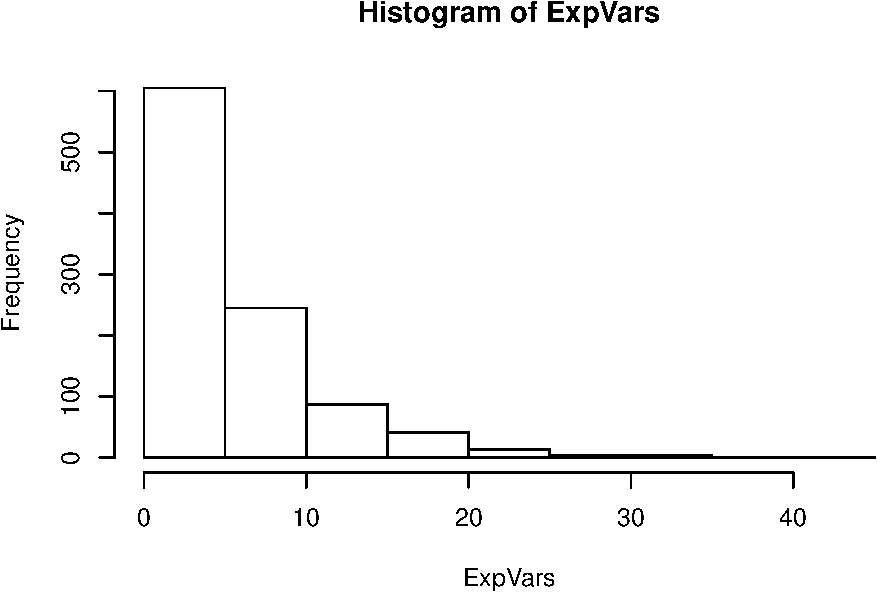
\includegraphics{SI-proj_files/figure-latex/unnamed-chunk-1-1.pdf}

To perform the actual simulation we use the following code which creates
1000 variables which are each the mean of 40 random \(x\) values such
that \(x \sim E(.2)\)

\begin{Shaded}
\begin{Highlighting}[]
\NormalTok{mns <-}\StringTok{ }\OtherTok{NULL}
\NormalTok{for (i in }\DecValTok{1} \NormalTok{:}\StringTok{ }\DecValTok{1000}\NormalTok{) mns <-}\StringTok{ }\KeywordTok{c}\NormalTok{(mns, }\KeywordTok{mean}\NormalTok{(}\KeywordTok{rexp}\NormalTok{(}\DecValTok{40}\NormalTok{, .}\DecValTok{2}\NormalTok{)))}
\KeywordTok{hist}\NormalTok{(mns)}
\end{Highlighting}
\end{Shaded}

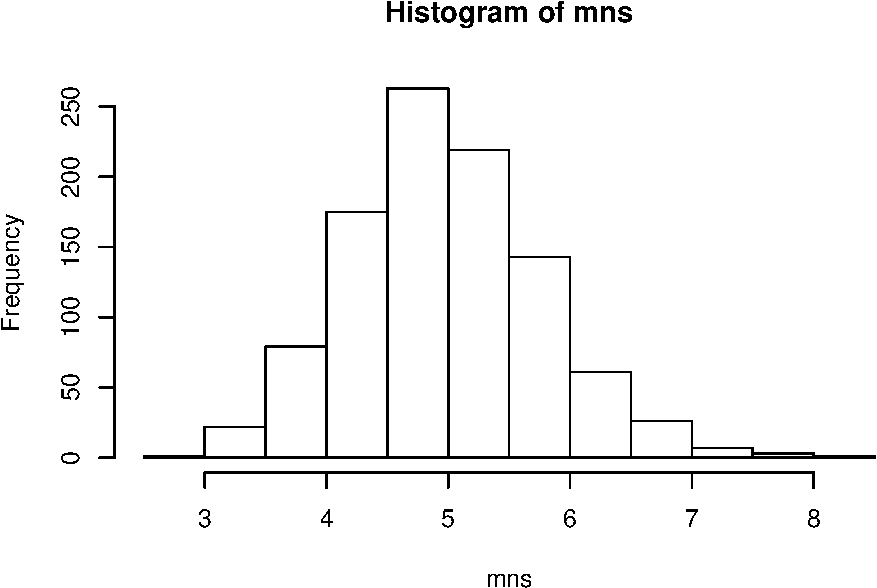
\includegraphics{SI-proj_files/figure-latex/unnamed-chunk-2-1.pdf} It is
already evident that this distribution of variables is approximately
normal based on its general shape.
\section{Sample Mean versus Theoretical Mean} The Theoretical Sample
mean is \(\mu_M = \mu\), that is the sample mean should be the same as
the distribution mean. For the Exponential Distribution,
\(E(x) = \frac{1}{\lambda} = \frac{1}{.2} = 5\). Using \(R\) to find the
sample mean, we see that the Sample mean is reasonably close to the
Theoretical Mean:

\begin{Shaded}
\begin{Highlighting}[]
\KeywordTok{mean}\NormalTok{(mns)}
\end{Highlighting}
\end{Shaded}

\begin{verbatim}
## [1] 4.9809
\end{verbatim}

Looking at the histogram for \texttt{mns}, it is clear that the
approximate normal curve is centered at about 5.

\section{Sample Variance versus Theoretical Variance}

The Theoretical Variance mean is given by
\(\sigma_M^2 = \frac{\sigma^2}{N-1}\) where \(N\) is the sample size.
For the Exponential Distribution,
\(Var(x) = \frac{1}{\lambda^2} = \frac{1}{.2^2} = 25\). Thus we have a
sample variance of
\(Var(x) = \sigma_M^2 = \frac{\sigma^2}{N-1} = \frac{25}{40 - 1} = .641\).
Using \(R\) to find the sample variance, we again see that the sample
variance is reasonably close to the Theoretical Variance:

\begin{Shaded}
\begin{Highlighting}[]
\KeywordTok{var}\NormalTok{(mns)}
\end{Highlighting}
\end{Shaded}

\begin{verbatim}
## [1] 0.632249
\end{verbatim}

Looking at the histogram for \texttt{mns}, it is clear that the
approximate normal curve has a variance of about .6.
\section{Conclusion} Thus we can see that the sample is following the
prescribed formulas and it is evident that the histogram of the sample
is essentially a normal distribution. Thus the Central Limit Theorem is
experimentally verifiy.

\end{document}
